\section{初步研究}



\subsection{定义}

\cpar{原生多模态模型 (NMMs):}  
从头开始同时在所有模态上训练的模型,不依赖于预训练的语言模型或视觉编码器。我们的重点是具有代表性的图像和文本模态,其中模型将文本和图像作为输入,并生成文本作为输出。

\cpar{早期融合:} 从一开始就启用多模态交互,几乎不使用模态特定的参数(例如,除了将图像块片化的线性层之外)。使用单一的 Transformer 模型,该方法处理原始多模态输入——词元化的文本和连续的图像块,而无需对图像进行离散化。我们将主要的 Transformer 称为解码器。

\cpar{晚融合:} 将多模态交互延迟到更深层,通常是在相互独立地处理每个模态的分离的单模态组件之后(例如,视觉编码器连接到大型语言模型)。

\cpar{模态无关路由:} 在稀疏混合专家中,\edit{模态无关}路由指的是依赖一个与模型联合训练的学成路由模块。

\cpar{模态感知路由:} 基于预定义规则的路由,例如基于模态类型(如视觉-词元、词元-词元)的路由。

\begin{table}[t!]
    \centering
    \setlength{\tabcolsep}{8pt}
    \renewcommand{\arraystretch}{1.0}
    \resizebox{1\linewidth}{!}{
    \begin{tabular}{c p{0.999\linewidth}}
         Expression & Definition  \\
         \shline
         \textbf{$N$}     & \normalfont{{Number of parameters in the multimodal decoder. For MoEs this refers to the \edit{active parameters.}}} \\
         \grayrow
         \textbf{$D$}     & \normalfont{{Total number of multimodal tokens.}} \\
         \textbf{$N_{v}$} & \normalfont{{Number of vision-only tokens.}} \\
         \grayrow
         \textbf{$D_{v}$} & \normalfont{{Number of parameters in the vision-specific encoder. Only exists in late-fusion architectures.}} \\
         \textbf{$C$}     & \small{{Total number of FLOPs, estimated as $C=6ND$ for early-fusion and $C=6(N_vD_v+ND)$ for late-fusion.}} \\
         \grayrow
         \textbf{$L$}     & \normalfont{{Average validation loss on interleaved image-text, image-caption, and text-only data mixtures.}} \\
    \end{tabular}}
    \caption{本文中使用的表达式的定义。}
    \label{tab:my_label}
\end{table}





\subsection{缩放律}
我们旨在理解NMMs的缩放属性以及不同的架构选择如何影响权衡。为此,我们在~\citet{kaplan2020scaling,
hoffmann2022training}提出的缩放定律框架内分析我们的模型。我们基于总参数数量计算浮点运算次数(FLOPs),采用与先验工作~\citep{hoffmann2022training,abnar2025parameters}相同的近似公式\(C = 6ND\)。然而,我们对这一估计进行了修改以适应我们的设置:对于晚期融合模型,FLOPs按照\(6(N_vD_v + ND)\)进行计算。
我们考虑一种设定,在给定计算预算\(C\)的情况下,目标是预测模型的最终\edit{损失},并确定最优的参数数量和训练词元数量。与LLM缩放相关的先前研究~\citep{hoffmann2022training}一致,我们假设最终模型的损失与模型大小(\(N\))和训练词元数量(\(D\))之间存在幂律关系:




\begin{equation}
\label{eq:scaling_laws}
    L = E + \frac{A}{N^{\alpha}} + \frac{B}{D^{\beta}}.
\end{equation}



\noindent 这里,\(E\) 表示在数据集上可实现的最低损失,而\(\frac{A}{N^{\alpha}}\) 捕获增加参数数量的效果,较大的模型会导致较低的损失,改进的速率由\(\alpha\) 控制。类似地,\(\frac{B}{D^{\beta}}\) 考虑了更多词元数量的好处,\(\beta\) 确定改进的速率。此外,我们假设计算预算(FLOPs)与\(N\) 和\(D\)(\(C \propto ND\) )之间存在线性关系。这进一步导致了\cref{tab:power_laws} 中详细说明的幂律关系。


\begin{figure}[t!]
    \centering
    \captionsetup{type=figure}
    \begin{subfigure}[t]{0.48\linewidth}
        \centering
        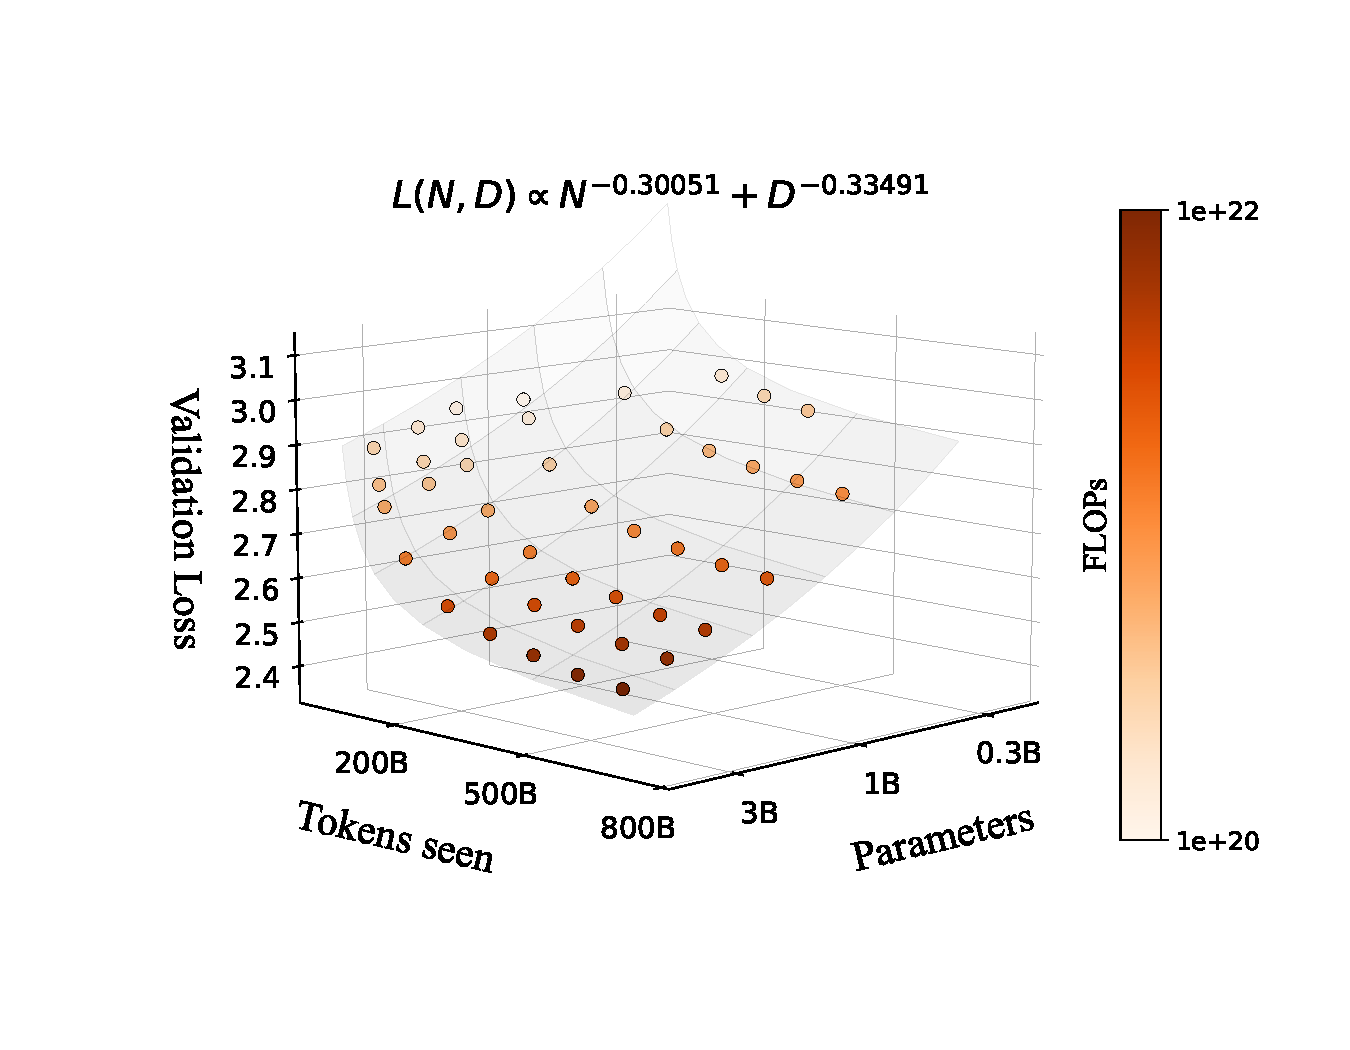
\includegraphics[width=1.02\linewidth]{assets/early/3d_scaling_early.pdf}
    \end{subfigure}
    \hfil
    \begin{subfigure}[t]{0.48\linewidth}
        \centering
        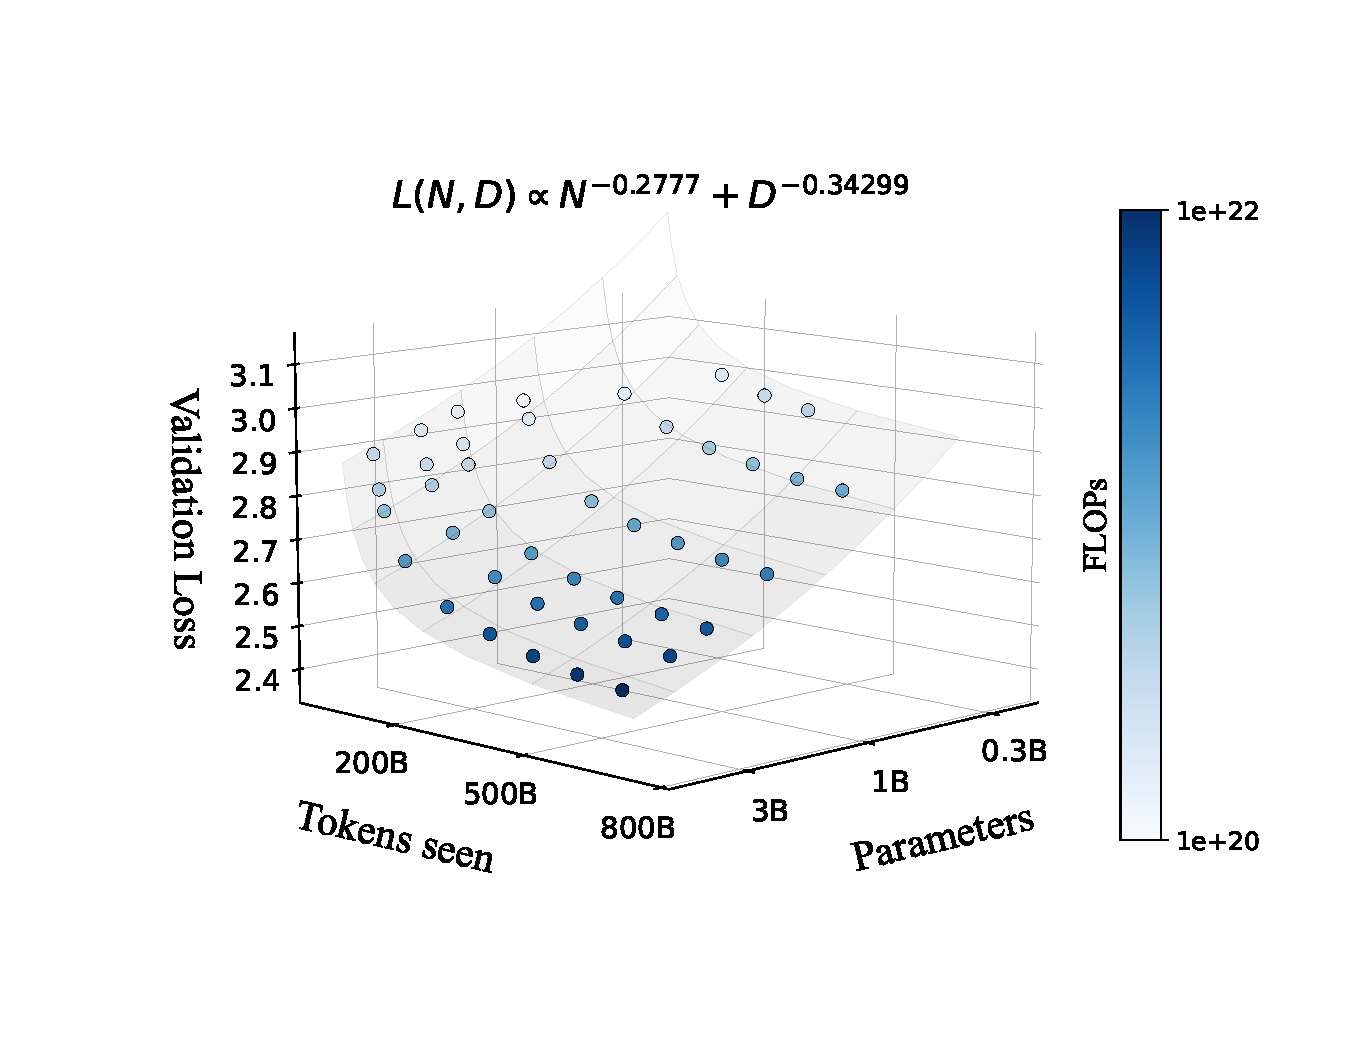
\includegraphics[width=1.02\linewidth]{assets/early/3d_scaling_late.pdf}
    \end{subfigure}
    \vspace{5pt}
    \setlength{\fboxsep}{0.5pt}
    \setlength{\fboxrule}{0pt}
    \caption{\textbf{原生多模态模型中 \fbox{\colorbox{CustomC_Light1!20}{\strut early-fusion}} 与 \fbox{\colorbox{CustomD_Light1!20}{late-fusion\strut}} 的尺度规律。} 每个点表示一个在不同 \edit{数量的} tokens(250M 到 400B)上训练的模型(300M 到 3B 参数)。我们报告了在 \edit{交错数据(Obelics)、图像描述数据(HQITP)和纯文本数据(DCLM)} 的验证集上的平均交叉熵损失。}
    \label{fig:early_vs_late_scaleflops_3d}
\end{figure}
        

\begin{table}[h]
    \centering
    \setlength{\tabcolsep}{16pt}
    \renewcommand{\arraystretch}{1}
    \resizebox{1\linewidth}{!}{
    \begin{tabular}{lccrc}
        Data type & dataset & \#samples & sampling prob. \\
         \shline
         \multirow{3}{*}{Image-Caption} &  DFN~\citep{fang2023data} & 2B & 27\%
         \\
          & COYO~{\citep{kakaobrain2022coyo700m}} &  600M & 11.25\% \\
          & HQITP  & 400M & 6.75\% \\
          Interleaved & Obelics \citep{laurenccon2024obelics}  & 141M Docs &
          45\% \\
          Text & DCLM \citep{li2024datacomp} & 6.6T Toks & 10\% \\
          
    \end{tabular}} \caption{\textbf{预训练数据混合。} 除非另有说明,训练混合物包含 45\%、45\% 和 10\% 的图像标题、交错文档和纯文本数据。}
    \label{tab:pretraining_datasets}
    \vspace{-5pt}
\end{table}

\subsection{实验装置}
\edit{Our models} are based on the autoregressive transformer
架构~\citep{vaswani2017attention} 配备 SwiGLU
前馈网络~\citep{shazeer2020glu} 和 QK-归一化~\citep{dehghani2023scaling}
后跟~\citet{li2024datacomp}。在早期融合模型中,图像块被线性投影以匹配文本词元的维度,而晚期融合则遵循 CLIP 架构~\citep{radford2021learning}。我们为文本词元采用因果注意力,为图像词元采用双向注意力,我们发现这种方法效果更好。训练在公共和私有多模态数据集的混合上进行,包括 DCLM \citep{li2024datacomp}、Obelics
\citep{laurenccon2024obelics}、DFN \citep{fang2023data}、COYO
\citep{kakaobrain2022coyo700m} 和一个私有的高质量图文对 (HQITP) 集合(见 \cref{tab:pretraining_datasets})。图像被调整为 224×224 分辨率,使用 14×14 的块大小。我们对多模态序列使用 1k 的上下文长度。为了提高训练效率,我们在 \texttt{bfloat16} 中训练我们的模型,完全分片数据并行 (FSDP)
\citep{zhao2023pytorch}、\edit{激活} 检查点和梯度累积。我们还对图像字幕数据集使用序列打包以减少填充词元的数量。类似于先前的工作~\citep{hoffmann2022training,aghajanyan2023scalingmm,abnar2025parameters},
我们在交错(Obelics)、图像字幕(HQITP)和纯文本数据(DCLM)的保留子集上评估性能。进一步的实现细节见~\cref{app:implementation_details}。
